\section{Resultados e discussões}

Os dados obtidos no experimento são mostrados na Tab. \ref{tab: dados}. 
Na Fig. \ref{fig: carga_vs_raio} é mostrada uma relação entre a carga e o raio calculados utilizando as equações \eqref{eq: r} e \eqref{eq: q'} para cada par $(t_s, t_d)$. 
Antecipando o resultado de que a carga em cada bolha será um multiplo inteiro de um valor fundamental $e=\qty{1,602e-19}{\coulomb}$ \cite{millikan}, a carga medida é dada em unidades dessa constante $e$.
 
\begin{figure}[h]
\centering
\caption{Carga vs raio da bolha}
\includegraphics[width=.9\linewidth]{imagens/Q_vs_R.eps}
\label{fig: carga_vs_raio}
\end{figure} 
 
\begin{table*}[t]
\centering
\caption{Dados obtidos no experimento.}
\resizebox{\textwidth}{!}{
\begin{tabular}{ccccc|ccccc|ccccc}
\toprule\midrule
\multicolumn{5}{c}{Parte 1} & \multicolumn{5}{c}{Parte 2} & \multicolumn{5}{c}{Parte 3} \\
$V$ & $t_s$ & $t_d$ & $r$ & $q$ &
$V$ & $t_s$ & $t_d$ & $r$ & $q$ &
$V$ & $t_s$ & $t_d$ & $r$ & $q$ \\
\multicolumn{1}{c}{$(\unit{\volt})$} &
\multicolumn{1}{c}{$\quad(\unit{\s})\quad$} &
\multicolumn{1}{c}{$(\unit{\s})$} &
\multicolumn{1}{c}{$(\qty{e-7}{\m})$} &
\multicolumn{1}{c}{$(\qty{e-19}{\coulomb})$} &
\multicolumn{1}{c}{$(\unit{\volt})$} &
\multicolumn{1}{c}{$\quad(\unit{\s})\quad$} &
\multicolumn{1}{c}{$(\unit{\s})$} &
\multicolumn{1}{c}{$(\qty{e-7}{\m})$} &
\multicolumn{1}{c}{$(\qty{e-19}{\coulomb})$} &
\multicolumn{1}{c}{$(\unit{\volt})$} &
\multicolumn{1}{c}{$\quad(\unit{\s})\quad$} &
\multicolumn{1}{c}{$(\unit{\s})$} &
\multicolumn{1}{c}{$(\qty{e-7}{\m})$} &
\multicolumn{1}{c}{$(\qty{e-19}{\coulomb})$} \\ 
\midrule
300 & 0,584 & 1,371 & 10,939 & 11,327 & 400 & 1,310 & 1,320 & 0,839 & 0,406 & 599 & 1,990 & 0,990 & 7,861 & 2,525 \\
300 & 0,461 & 0,558 & 6,775 & 11,382 & 400 & 2,270 & 2,730 & 3,006 & 0,771 & 599 & 1,210 & 1,620 & 5,046 & 1,547 \\
300 & 0,504 & 0,620 & 6,723 & 10,254 & 400 & 1,070 & 1,180 & 3,257 & 1,846 & 599 & 0,580 & 1,140 & 10,154 & 5,610 \\
300 & 0,486 & 0,575 & 6,227 & 10,025 & 400 & 1,100 & 1,060 & 2,044 & 1,204 & 599 & 2,470 & 1,880 & 3,933 & 0,782 \\
300 & 0,469 & 0,726 & 9,586 & 14,267 & 400 & 0,960 & 1,210 & 5,119 & 3,041 & 599 & 1,370 & 3,660 & 7,457 & 1,589 \\
300 & 3,150 & 3,870 & 2,681 & 0,655 & 400 & 1,130 & 1,220 & 2,819 & 1,528 & 599 & 1,620 & 2,190 & 4,423 & 1,009 \\
300 & 1,570 & 1,630 & 1,689 & 0,896 & 451 & 0,336 & 0,495 & 10,788 & 15,205 & 602 & 0,568 & 0,468 & 6,767 & 5,574 \\
300 & 1,190 & 1,850 & 6,041 & 3,538 & 451 & 0,363 & 0,726 & 12,949 & 15,094 & 602 & 0,602 & 0,502 & 6,347 & 4,900 \\
300 & 2,030 & 1,800 & 2,768 & 1,230 & 451 & 0,336 & 0,345 & 3,074 & 5,095 & 602 & 0,559 & 0,501 & 5,021 & 4,016 \\
400 & 0,690 & 0,900 & 6,416 & 5,225 & 451 & 0,336 & 0,540 & 11,700 & 15,934 & 602 & 0,534 & 0,435 & 7,203 & 6,350 \\
400 & 0,640 & 0,860 & 6,976 & 6,046 & 451 & 0,372 & 0,549 & 10,272 & 13,067 & 602 & 0,601 & 0,484 & 6,998 & 5,516 \\
400 & 0,680 & 0,860 & 6,121 & 5,127 & 500 & 1,390 & 1,170 & 4,058 & 1,625 & 602 & 0,586 & 0,571 & 2,336 & 1,707 \\
400 & 0,690 & 0,860 & 5,906 & 4,906 & 500 & 1,200 & 1,120 & 2,692 & 1,182 & 602 & 0,601 & 0,502 & 6,320 & 4,883 \\
400 & 0,890 & 1,370 & 6,923 & 4,081 & 500 & 1,220 & 1,170 & 2,065 & 0,880 & 602 & 0,569 & 0,540 & 3,390 & 2,586 \\
400 & 0,900 & 1,200 & 5,815 & 3,596 & 500 & 2,620 & 2,750 & 1,482 & 0,281 & 602 & 0,535 & 0,501 & 3,930 & 3,210 \\
400 & 1,150 & 1,280 & 3,279 & 1,722 & 500 & 1,090 & 2,480 & 7,912 & 2,659 & 602 & 0,835 & 0,970 & 4,505 & 2,121 \\
400 & 0,570 & 0,640 & 4,833 & 5,099 & 500 & 0,950 & 1,680 & 7,462 & 3,129 & 602 & 0,803 & 1,070 & 6,151 & 2,833 \\
400 & 0,720 & 0,830 & 4,734 & 3,905 & 551 & 0,806 & 1,221 & 7,165 & 3,407 & 602 & 0,835 & 1,070 & 5,659 & 2,550 \\
400 & 1,400 & 2,560 & 6,277 & 2,206 & 551 & 0,814 & 1,187 & 6,855 & 3,278 & 602 & 0,802 & 1,103 & 6,436 & 2,929 \\
400 & 1,070 & 1,770 & 6,708 & 3,199 & 551 & 1,151 & 1,372 & 4,128 & 1,523 & 602 & 0,768 & 1,069 & 6,681 & 3,159 \\
400 & 1,170 & 1,580 & 5,196 & 2,459 & 551 & 0,806 & 1,354 & 7,819 & 3,573 & 602 & 0,769 & 1,103 & 6,924 & 3,229 \\
400 & 1,120 & 1,490 & 5,195 & 2,584 & 551 & 1,063 & 1,159 & 3,080 & 1,283 & 602 & 0,735 & 1,103 & 7,434 & 3,562 \\
\midrule\bottomrule
\end{tabular}
}
\label{tab: dados}
\end{table*}
 
 
Foi calculado o valor médio da distância entre um ponto e o múltiplo inteiro de $e$ mais próximo, e foi encontrado o valor de $\Delta q = 0,233\,e$. 
Os pontos em que $ne - \Delta q \leq q \leq ne + \Delta q,\, n \in \mathbb{N}$, estão destacados em preto na Fig. \ref{fig: carga_vs_raio}, enquanto	que os demais estão em vermelho. 
Ou seja, os pontos em vermelho são aqueles que desviam consideravelmente do valores teoricamente permitidos para a carga.

É possível ver na Fig. \ref{fig: carga_vs_raio} que os pontos tendem a se agrupar em torno de múltiplos inteiros de $e$, indicados pelas linhas horizontais tracejadas. 
Embora haja muitos pontos vermelhos, nota-se que a medida que os valores de $q$ aumentam, a razão entre pontos vermelhos e pretos diminui. 
Isso se dá provavelmente porque quanto menores são os valores numéricos das medidas, maior é a incerteza.
 
Assim, os dados obtidos corroboram a hipótese de que as cargas ocorrem em múltiplos inteiros de $e$. 
No entanto, a baixa quantidade de pontos com $q$ alto torna difícil uma conclusão assertiva. 
Portanto, faz-se necessário realizar mais medições para obter tais pontos.

Assumindo agora que $q = ne$, mas com $e$ sendo algum valor desconhecido, é possível utilizar os dados obtidos para estimar o valor numérico de $e$. Para cada valor de $q$, foi associado um número natural $n$, obtido ao arredondar $q/(\qty{1,602e19}{\coulomb})$. 
Na Fig. \ref{fig: carga_vs_n}, é mostrada a relação entre $q$ e $n$. Realizando uma regressão linear, foi obtido o coeficiente angular $e = \qty{1,658e-19}{\coulomb}$.

Comparando com o valor dado pela literatura \cite{millikan} de $e = \qty{1,602e-19}{\coulomb}$, o valor calculado tem um desvio percentual de aproximadamente $3\%$, que é um resultado satisfatório.


\begin{figure}
\centering
\caption{Carga vs n}
\includegraphics[width=.9\linewidth]{imagens/q_vs_napprox.eps}
\label{fig: carga_vs_n}
\end{figure}

